\begin{figure}[h]
	\centering
	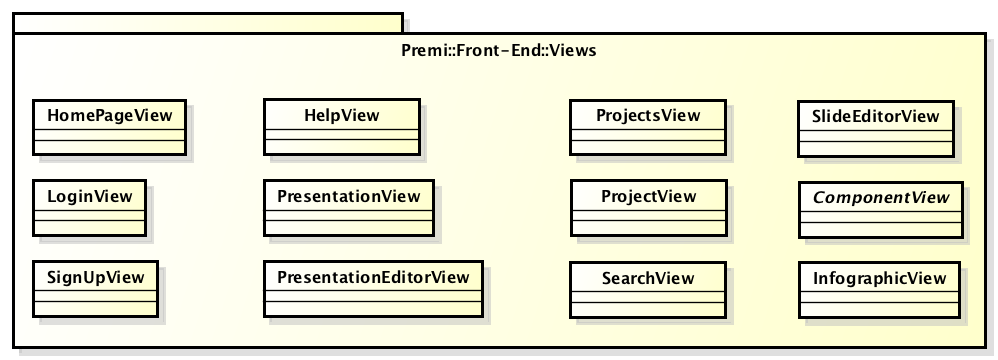
\includegraphics[width=0.7\linewidth]{img/premi_front_end_views}
	\caption[Premi::Front-End::Views]{Premi::Front-End::Views}
\end{figure}
Il package gestisce le view del front-end dell'applicazione. Comunica con il model, il controller e le direttive della struttura per acquisire i dati da visualizzare e far ottenere al model i dati modificati dall'utente attraverso il controller. Il package inoltre comunica con i framework esterni necessari per la creazione degli oggetti da utilizzare nel programma.

\subsubsection{Component}
	\begin{figure}[h]
		\centering
		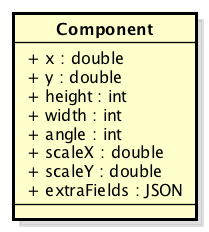
\includegraphics[width=0.3\linewidth]{img/premi_front_end_views_component}
		\caption[Premi::Front-End::Views::Component]{Premi::Front-End::Views::Component}
	\end{figure}
	
	\paragraph{Descrizione}
	Visualizza i componenti che è possibile inserire in una slide e le rispettive informazioni.
	
	\paragraph{Utilizzo}
	Viene utilizzata come view per visualizzare e modificare gli attributi di un componente della slide. Da essa derivano le view specifiche di ciascun componente.
	
	\paragraph{Relazioni con altre classi}
	\begin{itemize}
		\item \textbf{\textit{IN} ComponentCtrl}:\\
		Classe che gestisce le operazioni generali per la gestione di un componente.
	\end{itemize}
	
	\paragraph{Attributi}
	\begin{itemize}
		\item \textbf{+ x: double}:\\
			Campo dati che contiene la coordinata x di origine del componente;
		\item \textbf{+ y: double}:\\
			Campo dati che contiene la coordinata y di origine del componente;
		\item \textbf{+ height: int}:\\
			Campo dati che contiene la l'altezza del componente;
		\item \textbf{+ width: int}:\\
			Campo dati che contiene la larghezza del componente;
		\item \textbf{+ angle: int}:\\
			Campo dati che contiene l'angolo di rotazione del componente;
		\item \textbf{+ scaleX: duble}:\\
			Campo dati che contiene la scala sull'asse x del componente;
		\item \textbf{+ scaleY: double}:\\
			Campo dati che contiene la scala sull'asse y del componente;
		\item \textbf{+ extraFields: JSON}:\\
			Campo dati che contiene un array JSON avente tutti i campi dati secondari di un componente.
	\end{itemize}
\newpage
	

%\subsubsection{Help}
%	\begin{figure}[h]
%		\centering
%		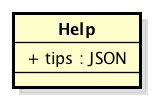
\includegraphics[width=0.3\linewidth]{img/premi_front_end_views_help}
%		\caption[Premi::Front-End::Views::Help]{Premi::Front-End::Views::Help}
%	\end{figure}
%	
%	\paragraph{Descrizione}
%	View che contiene il tool di aiuto all'utente.
%	
%	\paragraph{Utilizzo}
%	Viene utilizzata come view per visualizzare l'help per l'utente.
%	
%	\paragraph{Relazioni con le altre classi}
%	\begin{itemize}
%		\item \textbf{\textit{IN} HelpCtrl}:\\
%		Classe che gestisce la visualizzazione dell'aiuto all'utente.
%	\end{itemize}
%	
%	\paragraph{Attributi}
%	\begin{itemize}
%		\item \textbf{+ tips:JSON}: \\
%		Campo dati che contiene un array JSON con tutti gli aiuti da fornire all'utente.
%	\end{itemize}
%\newpage
	
	
\subsubsection{HomePage}
	\begin{figure}[h]
		\centering
		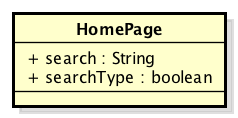
\includegraphics[width=0.3\linewidth]{img/premi_front_end_views_homepage}
		\caption[Premi::Front-End::Views::HomePage]{Premi::Front-End::Views::HomePage}
	\end{figure}
	
	\paragraph{Descrizione}
	Visualizza la pagina principale dell'applicazione.
	
	\paragraph{Utilizzo}
	Viene utilizzata come view per accedere all'area riservata all'utente, alle pagine per il login e la registrazione ed è utilizzata per cercare un utente o un progetto nel sistema attraverso l'apposito form.
	
	\paragraph{Relazioni con le altre classi}
	\begin{itemize}
		\item \textbf{\textit{IN} HomePageCtrl}:\\
			Classe che gestisce la home page e gli accessi alle altre pagine dell'applicazione;
		\item \textbf{\textit{IN} SearchCtrl}:\\
			Classe che gestisce le operazioni di ricerca;
		\item \textbf{\textit{IN} HelpCtrl}:\\
			Classe che gestisce le operazioni per l'aiuto all'utente;
		\item \textbf{\textit{IN} AuthenticationCtrl}:\\
			Classe che gestisce le operazioni per l'autenticazione dell'utente.
	\end{itemize}
	
	\paragraph{Attributi}
	\begin{itemize}
		\item \textbf{+ search: String}:\\
			Campo dati per il contenuto della ricerca da effettuare;
		\item \textbf{+ searchType: boolean}:\\
			Campo dati la scelta del tipo di ricerca da effettuare (per nome utente o per nome del progetto).
	\end{itemize}
\newpage
	
	
\subsubsection{InfographicEditor}
	\begin{figure}[h]
		\centering
		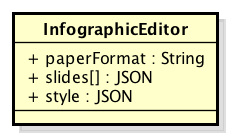
\includegraphics[width=0.3\linewidth]{img/premi_front_end_views_infographiceditor}
		\caption[Premi::Front-End::Views::InfographicEditor]{Premi::Front-End::Views::InfographicEditor}
	\end{figure}
	
	\paragraph{Descrizione}
	Visualizza la pagina per la gestione di un'infografica.
	
	\paragraph{Utilizzo}
	Viene utilizzata come view per visualizzare un'infografica, modificarla e salvarla.
	
	\paragraph{Relazioni con le altre classi}
	\begin{itemize}
		\item \textbf{\textit{IN} InfographicEditorCtrl}:\\
			Classe che gestisce le operazioni per le infografiche (creazione, modifica, salvataggio);
		\item \textbf{\textit{IN} HelpCtrl}:\\
			Classe che gestisce le operazioni per l'aiuto all'utente.
	\end{itemize}
	
	\paragraph{Attributi}
	\begin{itemize}
		\item \textbf{+ paperFormat: String}:\\
			Campo dati per il formato adottato dall'infografica;
		\item \textbf{+ slides[]: JSON}:\\
			Campo dati contenente l'array di slide che compongono l'infografica;
		\item \textbf{+ style: JSON}:\\
		Campo dati per le informazioni dello stile da utilizzare per l'infografica.
	\end{itemize}
\newpage
	
	
\subsubsection{Login}
	\begin{figure}[h]
		\centering
		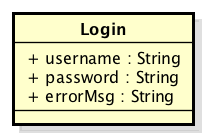
\includegraphics[width=0.3\linewidth]{img/premi_front_end_views_login}
		\caption[Premi::Front-End::Views::Login]{Premi::Front-End::Views::Login}
	\end{figure}
	
	\paragraph{Descrizione}
	View che visualizza il form per inserire i dati necessari al login. Fornisce inoltre un link per il reset della password.
	
	\paragraph{Utilizzo}
	Viene visualizzata dopo aver premuto il rispettivo bottone per permettere l'autenticazione all'utente.
	
	\paragraph{Relazioni con le altre classi}
	\begin{itemize}
		\item \textbf{\textit{IN} LoginCtrl}:\\
		Classe che gestisce le operazioni per l'autenticazione al sito;
		\item \textbf{\textit{IN} AuthenticationCtrl}:\\
		Classe che gestisce le operazioni per l'autenticazione dell'utente.
	\end{itemize}
	
	\paragraph{Attributi}
	\begin{itemize}
		\item \textbf{+ username: String}:\\
		Campo dati contenente lo username dell'utente;
		\item \textbf{+ password: String}:\\
		Campo dati per la password dell'utente;
		\item \textbf{+ errorMsg: String}:\\
		Campo dati contenente l'eventuale messaggio di errore da fornire all'utente.
	\end{itemize}
\newpage


\subsubsection{MyAccount}
	\begin{figure}[h]
		\centering
		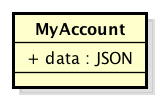
\includegraphics[width=0.3\linewidth]{img/premi_front_end_views_myaccount}
		\caption[Premi::Front-End::Views::MyAccount]{Premi::Front-End::Views::MyAccount}
	\end{figure}
	
	\paragraph{Descrizione}
	View che visualizza le informazioni personali dell'utente.
	
	\paragraph{Utilizzo}
	Viene visualizzata dopo aver eseguito il login per mostrare le informazioni personali dell'utente.
	
	\paragraph{Relazioni con le altre classi}
	\begin{itemize}
		\item \textbf{\textit{IN} MyAccountCtrl}:\\
		Classe che gestisce le operazioni per il recupero dei dati dell'utente.
	\end{itemize}
	
	\paragraph{Attributi}
	\begin{itemize}
		\item \textbf{+ data: JSON}:\\
		Campo dati contenente i dati dell'utente.
	\end{itemize}
\newpage
	
	
\subsubsection{PresentationEditor}
	\begin{figure}[h]
		\centering
		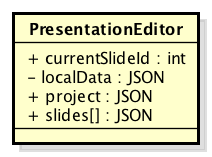
\includegraphics[width=0.3\linewidth]{img/premi_front_end_views_presentationeditor}
		\caption[Premi::Front-End::Views::PresentationEditor]{Premi::Front-End::Views::PresentationEditor}
	\end{figure}
	
	\paragraph{Descrizione}
	Visualizza l'editor di una presentazione.
	
	\paragraph{Utilizzo}
	Viene utilizzata come view per modificare una presentazione e le impostazioni globali di essa. Permette di aggiungere o rimuovere slide e di spostarsi tra di esse. Dà la possibilità, inoltre, di accedere alla sezione di modifica di ogni singola slide.
	
	\paragraph{Relazioni con le altre classi}
	\begin{itemize}
		\item \textbf{\textit{IN} PresentationEditorCtrl}:\\
		Classe che gestisce le operazioni di modifica delle impostazioni generali della presentazione e le operazioni di spostamento, aggiunta e rimozione di una slide;
		\item \textbf{\textit{IN} AuthenticationCtrl}:\\
		Classe che gestisce le operazioni per l'autenticazione dell'utente.
	\end{itemize}
	
	\paragraph{Attributi}
	\begin{itemize}
		\item \textbf{+ project: JSON}:\\
		Campo dati che contiene le informazioni del progetto corrente;
		\item \textbf{+ slides[]: JSON}:\\
		Campo dati che contiene un array JSON avente le principali informazioni delle slide della presentazione;
		\item \textbf{+ currentSlideId: int}:\\
		Campo dati che contiene l'id della slide corrente;
		\item \textbf{- localData: JSON}:\\
		Campo dati che contiene le informazioni relative agli indici della slide corrente e agli indici massimi della presentazione.
	\end{itemize}
\newpage
	
	
\subsubsection{Presentation}
	\begin{figure}[h]
		\centering
		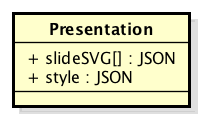
\includegraphics[width=0.3\linewidth]{img/premi_front_end_views_presentation}
		\caption[Premi::Front-End::Views::Presentation]{Premi::Front-End::Views::Presentation}
	\end{figure}
	
	\paragraph{Descrizione}
	Visualizza la pagina di visualizzazione di una presentazione.
	
	\paragraph{Utilizzo}
	Viene utilizzata come view per visualizzare e riprodurre la presentazione, sia come ascoltatore che come presentatore.
	
	\paragraph{Relazioni con le altre classi}
	\begin{itemize}
		\item \textbf{\textit{IN} PresentationCtrl}:\\
			Classe che gestisce le operazioni di recupero dei dati e della visualizzazione della presentazione.
	\end{itemize}
	
	\paragraph{Attributi}
	\begin{itemize}
		\item \textbf{+ slideSVG[]: String}:\\
		Campo dati che contiene un array di stringhe di oggetti SVG rappresentanti le slide della presentazione;
		\item \textbf{+ style: JSON}: \\
		Campo dati che contiene un oggetto JSON con i dati dello stile della presentazione (tema e effetto di transizione).
	\end{itemize}
\newpage
	
	
\subsubsection{Projects}
	\begin{figure}[h]
		\centering
		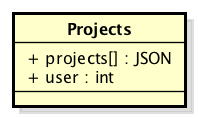
\includegraphics[width=0.3\linewidth]{img/premi_front_end_views_projects}
		\caption[Premi::Front-End::Views::Projects]{Premi::Front-End::Views::Projects}
	\end{figure}
	
	\paragraph{Descrizione}
	Visualizza la pagina con la lista dei progetti di un utente.
	
	\paragraph{Utilizzo}
	Viene utilizzata come view per selezionare i progetti di utente da aprire e per accedere alla funzione di crearne uno nuovo.
	
	\paragraph{Relazioni con le altre classi}
	\begin{itemize}
		\item \textbf{\textit{IN} NewProject}:\\
			Classe che gestisce la creazione di un nuovo progetto;
		\item \textbf{\textit{IN} ProjectsCtrl}:\\
			Classe che gestisce il caricamento dei progetti di un utente e le operazioni che è possibile effettuare su di essi;
		\item \textbf{\textit{IN} HelpCtrl}:\\
		Classe che gestisce le operazioni per l'aiuto all'utente.
	\end{itemize}
	
	\paragraph{Attributi}
	\begin{itemize}
		\item \textbf{+ projects[]: JSON}:\\
			Campo dati che contiene l'array dei progetti dell'utente;
		\item \textbf{+ user: int}:\\
			Campo dati che contiene l'id dell'utente.
	\end{itemize}
\newpage
	
	
\subsubsection{Project}
	\begin{figure}[h]
		\centering
		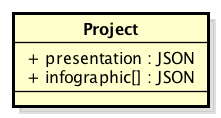
\includegraphics[width=0.3\linewidth]{img/premi_front_end_views_project}
		\caption[Premi::Front-End::Views::Project]{Premi::Front-End::Views::Project}
	\end{figure}
	
	\paragraph{Descrizione}
	Visualizza l'anteprima del progetto selezionato.
	
	\paragraph{Utilizzo}
	Viene utilizzata come view per visualizzare l'anteprima della presentazione e le infografiche di un progetto e per selezionare le operazioni da eseguire su di essi.
	
	\paragraph{Relazioni con le altre classi}
	\begin{itemize}
		\item \textbf{\textit{IN} ProjectsCtrl}:\\
			Classe che gestisce i progetti di un utente;
		\item \textbf{\textit{OUT} PresentationCtrl}:\\
			Classe che gestisce la visualizzazione di una presentazione;
		\item \textbf{\textit{OUT} presentationEditorCtrl}:\\
			Classe che gestisce la modifica di una presentazione;
		\item \textbf{\textit{OUT} infographicEditorCtrl}:\\
			Classe che gestisce le infografiche e la loro modifica;
		\item \textbf{\textit{IN} AuthenticationCtrl}:\\
			Classe che gestisce le operazioni per l'autenticazione dell'utente.
	\end{itemize}
	
	\paragraph{Attributi}
	\begin{itemize}
		\item \textbf{+ presentation: JSON}:\\
			Campo dati che contiene un oggetto JSON avente l'id e i dati relativi all'anteprima del progetto;
		\item \textbf{+ infographic[]: JSON}:\\
			Campo dati che contiene un array di oggetti JSON aventi gli id e i dati relativi alle infografiche del progetto.
	\end{itemize}
\newpage
	
	
\subsubsection{ResetPassword}
	\begin{figure}[h]
		\centering
		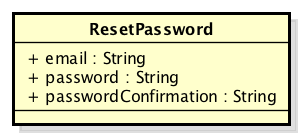
\includegraphics[width=0.3\linewidth]{img/premi_front_end_views_resetpassword}
		\caption[Premi::Front-End::Views::ResetPassword]{Premi::Front-End::Views::ResetPassword}
	\end{figure}
	
	\paragraph{Descrizione}
	View che contiene il form per procedere con il reset della password.
	
	\paragraph{Utilizzo}
	Viene utilizzata come view per resettare la password dopo aver avviato l'apposita procedura di reset.
	
	\paragraph{Relazioni con le altre classi}
	\begin{itemize}
		\item \textbf{\textit{IN} ResetPasswordCtrl}:\\
		Classe che gestisce il reset della password di un utente.
	\end{itemize}
	
	\paragraph{Attributi}
	\begin{itemize}
		\item \textbf{+ email:String}: \\
		Campo dati che contiene l'email dell'utente che deve resettare la password;
		\item \textbf{+ password:String}: \\
		Campo dati che contiene la nuova password per l'utente;
		\item \textbf{+ passwordConfirmation:String}: \\
		Campo dati che contiene la conferma della nuova password per l'utente.
	\end{itemize}
\newpage
	

\subsubsection{Search}
	\begin{figure}[h]
		\centering
		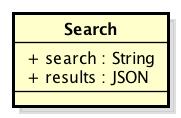
\includegraphics[width=0.3\linewidth]{img/premi_front_end_views_search}
		\caption[Premi::Front-End::Views::Search]{Premi::Front-End::Views::Search}
	\end{figure}
	
	\paragraph{Descrizione}
	View che visualizza i risultati di una ricerca eseguita da un utente, lanciata dalla schermata di home page.
	
	\paragraph{Utilizzo}
	Viene utilizzata come view per visualizzare i risultati di una ricerca.
	
	\paragraph{Relazioni con le altre classi}
	\begin{itemize}
		\item \textbf{\textit{IN} SearchCtrl}:\\
		Classe che gestisce la ricerca per nome utente o per nome del progetto.
	\end{itemize}
	
	\paragraph{Attributi}
	\begin{itemize}
		\item \textbf{+ search: String}:\\
		Campo dati per identificare il nome utente o il nome del progetto da cercare;
		\item \textbf{+ results: JSON}:\\
		Campo dati che contiene un array JSON con i risultati della ricerca;
	\end{itemize}
\newpage
	
	
\subsubsection{SignUp}
	\begin{figure}[h]
		\centering
		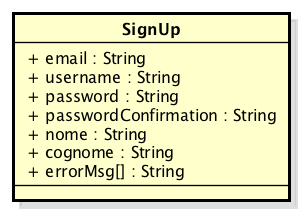
\includegraphics[width=0.3\linewidth]{img/premi_front_end_views_signup}
		\caption[Premi::Front-End::Views::SignUp]{Premi::Front-End::Views::SignUp}
	\end{figure}
	
	\paragraph{Descrizione}
	View che visualizza il form per permettere la registrazione dell'utente al sito.
	
	\paragraph{Utilizzo}
	Viene utilizzata come view per inserire i dati necessari a registrarsi nel sistema.
	
	\paragraph{Relazioni con le altre classi}
	\begin{itemize}
		\item \textbf{\textit{IN} SignUpCtrl}:\\
		Classe che gestisce le operazioni di registrazione al sito;
		\item \textbf{\textit{IN} AuthenticationCtrl}:\\
		Classe che gestisce le operazioni per l'autenticazione dell'utente.
	\end{itemize}
	
	\paragraph{Attributi}
	\begin{itemize}
		\item \textbf{+ email: String}:\\
			Campo dati per l'email dell'utente;
		\item \textbf{+ username: String}:\\
			Campo dati per il nome utente;
		\item \textbf{+ password: String}:\\
			Campo dati per la password dell'utente;
		\item \textbf{+ passwordConfirmation: String}:\\
			Campo dati per la ripetizione della password dell'utente;
		\item \textbf{+ Nome: String}:\\
			Campo dati per il nome dell'utente;
		\item \textbf{+ Cognome: String}:\\
			Campo dati per il cognome dell'utente;		
		\item \textbf{+ errorMsg[]: String}:\\
			Array contenente gli eventuali messaggi di errore da fornire all'utente se i dati non sono inseriti correttamente.
	\end{itemize}
\newpage
	
	
\subsubsection{SlideEditor}
	\begin{figure}[h]
		\centering
		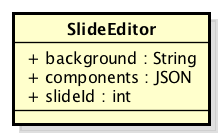
\includegraphics[width=0.3\linewidth]{img/premi_front_end_views_slideeditor}
		\caption[Premi::Front-End::Views::SlideEditor]{Premi::Front-End::Views::SlideEditor}
	\end{figure}
	
	\paragraph{Descrizione}
	Visualizza la sezione dedicata alla modifica di una slide della presentazione.
	
	\paragraph{Utilizzo}
	Viene utilizzata come view per modificare una slide, permette di inserire i componenti, modificarli secondo i rispettivi parametri e rimuoverli. Permette inoltre di salvare le modifiche effettuate.
	
	\paragraph{Relazioni con le altre classi}
	\begin{itemize}
		\item \textbf{\textit{IN} HelpCtrl}:\\
			Classe che gestisce le operazioni per l'aiuto all'utente;
		\item \textbf{\textit{IN} SlideEditorCtrl}:\\
			Classe che gestisce le operazioni di modifica di una slide, la gestione dei suoi componenti e il suo salvataggio;
		\item \textbf{\textit{IN} PresentationEditorCtrl}:\\
			Classe che gestisce le operazioni di modifica delle impostazioni generali della presentazione e le operazioni di spostamento, aggiunta e rimozione di una slide.
	\end{itemize}
	
	\paragraph{Attributi}
	\begin{itemize}
		\item \textbf{+ background: String}:\\
			Campo dati per il background della slide;
		\item \textbf{+ components[]: JSON}:\\
			Campo dati contenente un array con tutti gli elementi presenti nella slide;
		\item \textbf{+ slideId: int}:\\
			Campo dati per l'id della slide corrente.
	\end{itemize}